\documentclass[11pt,a4paper]{ivoa}
\input tthdefs

\usepackage[utf8]{inputenc}

\title{Astronomical Data Query Language}

\ivoagroup{Data Access Layer Working Group}

\author[http://wiki.ivoa.net/twiki/bin/view/IVOA/IvoaVOQL]{The IVOA Virtual Observatory Query Language (VOQL) working group members}
\author[http://wiki.ivoa.net/twiki/bin/view/IVOA/IvoaDAL]{The IVOA Data Access Layer (DAL) working group members}

\editor[http://wiki.ivoa.net/twiki/bin/view/IVOA/DaveMorris]{Dave Morris}

\previousversion[http://www.ivoa.net/Documents/ADQL/2.0]{ADQL-2.0}

\begin{document}

\begin{abstract}
This document describes the Astronomical Data Query Language (ADQL).
ADQL has been developed based on SQL92.
This document describes the subset of the SQL grammar supported by ADQL.
Special restrictions and extensions to SQL92 have been defined in order
to support generic and astronomy specific operations.
\end{abstract}

\section*{Acknowledgments}

The authors would like to acknowledge all contributors to this and previous 
versions of this standard, especially:
P. Dowler,
J. Lusted,
M. A. Nieto-Santisteban,
W. O'Mullane,
M. Ohishi,
I. Ortiz,
P. Osuna,
Y Shirasaki,
and
A. Szalay.

\section*{Conformance-related definitions}

The words ``MUST'', ``SHALL'', ``SHOULD'', ``MAY'', ``RECOMMENDED'', and
``OPTIONAL'' (in upper or lower case) used in this document are to be
interpreted as described in IETF standard, \citet{std:RFC2119}.

The \emph{Virtual Observatory (VO)} is general term for a collection of 
federated resources that can be used to conduct astronomical research, 
education, and outreach. The \href{http://www.ivoa.net}{International
Virtual Observatory Alliance (IVOA)} is a global collaboration of separately 
funded projects to develop standards and infrastructure that enable VO 
applications.

\section{Introduction}

The Astronomical Data Query Language (ADQL) is the language used by the
International Virtual Observatory Alliance (IVOA) to represent astronomy queries
posted to VO services. The IVOA has developed several standardized protocols
to access astronomical data, e.g., SIAP and SSAP for image and spectral data
respectively. These protocols might be satisfied using a single table query.
However, different VO services have different needs in terms of query complexity
and ADQL arises in this context.

The ADQL specification makes no distinction between core and advanced or
extended functionalities. Hence ADQL has been built according to a single
language definition (BNF based [1]). Any service making use of ADQL would
then define the level of compliancy to the language. This would allow the notion
of core and extension to be service-driven and it would decouple the language
from the service specifications.

ADQL is based on the Structured Query Language (SQL), especially on SQL 92.
The VO has a number of tabular data sets and many of them are stored in
relational databases, making SQL a convenient access means. A subset of the
SQL grammar has been extended to support queries that are specific to
astronomy. Similarly to SQL, the ADQL language definition is not semantically
safe by design and therefore this specification defines syntactical correctness
only. Type safety has been achieved as far as it can be done in SQL.
The exact meaning of key words indicating requirement levels can be found in
the References section [2].

\subsection{Role within the VO Architecture}

\begin{figure}
\centering
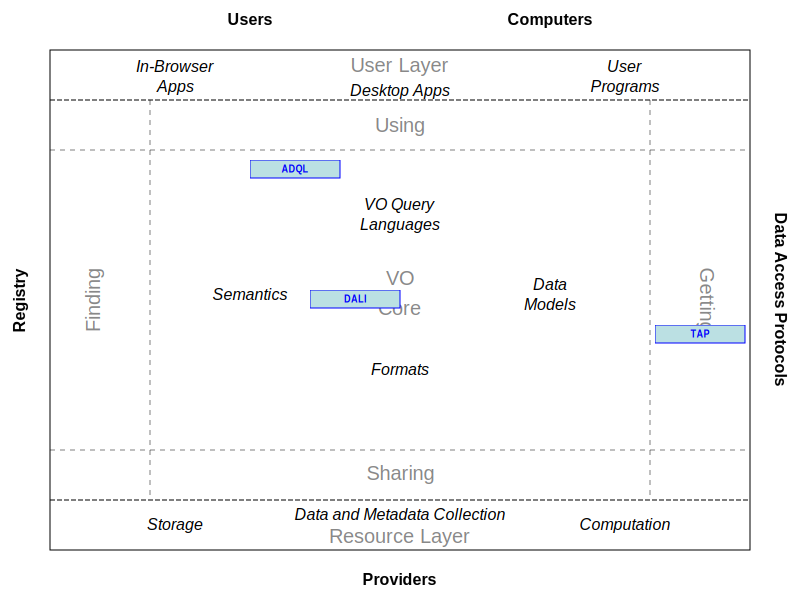
\includegraphics[width=0.9\textwidth]{archdiag.png}
\caption{Architecture diagram for this document}
\label{fig:archdiag}
\end{figure}

Fig.~\ref{fig:archdiag} shows the role this document plays within the
IVOA architecture \citep{note:VOARCH}.

\appendix

\section{Changes from Previous Versions}

\subsection{Changes from ADQL-2.0}




\bibliography{ivoatex/ivoabib}

\end{document}

